\documentclass[12pt]{beamer}

\usetheme{Oxygen}
\usepackage{thumbpdf}
\usepackage{wasysym}
% \usepackage{ucs}
\usepackage[utf8]{inputenc}
\usepackage{pgf,pgfarrows,pgfnodes,pgfautomata,pgfheaps,pgfshade}
\usepackage{verbatim}
\usepackage{multicol}


\pdfinfo
{
  /Title       (Taller de Desarrollo Web)
  /Creator     (TeX)
  /Author      (Sebastián Salazar Molina)
}


\title{Taller de Desarrollo Web}
\subtitle{Laravel}
\author{Sebastián Salazar Molina.}
\institute[INF - UTEM] { Unidad de Informática - Universidad Tecnológica Metropolitana }
\date{27 de Abril de 2014}

\begin{document}

\frame{\titlepage}

\section*{}
\begin{frame}
  \frametitle{Contenidos}
  \begin{multicols}{2}
    \tableofcontents[section=1,hidesubsections]
  \end{multicols}
\end{frame}

\AtBeginSection[]
{
  \frame<handout:0>
  {
    \frametitle{Contenidos}
    \begin{multicols}{2}
    \tableofcontents[currentsection,hideallsubsections]
    \end{multicols}
  }
}

\AtBeginSubsection[]
{
  \frame<handout:0>
  {
    \frametitle{Contenidos}
%     \begin{multicols}{2}
    \tableofcontents[sectionstyle=show/hide,subsectionstyle=show/shaded/hide]
%     \end{multicols}
  }
}

\newcommand<>{\highlighton}[1]{%
  \alt#2{\structure{#1}}{{#1}}
}

\newcommand{\icon}[1]{\pgfimage[height=1em]{#1}}



%%%%%%%%%%%%%%%%%%%%%%%%%%%%%%%%%%%%%%%%%
%%%%%%%%%% Content starts here %%%%%%%%%%
%%%%%%%%%%%%%%%%%%%%%%%%%%%%%%%%%%%%%%%%%



% Introducción
\section{Introducción}
\subsection{Introducción}

\begin{frame}
\frametitle{Acerca de mí.}
\begin{itemize}
 \item<2-> Sebastián Alexis Salazar Molina (@sebastian\_sm) .
 \item<3-> Ingeniero Civil en Computación (UTEM).
 \item<4-> Consultor TI en \href{http://www.experti.cl}{ExperTI} (C/C++ , PHP, Java)
 \item<5-> \href{http://sebastian.cl}{http://sebastian.cl}
\end{itemize}
\end{frame}


\begin{frame}
\frametitle{Acerca del taller.}

Este taller está pensado para personas sin conocimientos previos y es una aproximación muy básica e inicial hacia el desarrollo web, usando el framework Laravel.
\end{frame}


\begin{frame}
\frametitle{Temas}
Los temas que se trataremos son:
\begin{itemize}
 \item<1-> Herramientas.
 \item<2-> Servidores Web.
 \item<3-> HTML / CSS.
 \item<4-> JavaScript / jQuery.
 \item<5-> PHP.
 \item<6-> SQL / PostgreSQL.
 \item<7-> Laravel.
\end{itemize}
\end{frame}

\section{Herramientas}

\subsection{Computador}

\begin{frame}
 \frametitle{Computador}
 La principal herramienta del Desarrollador, es su \alert{computador}.
 \newline
 Deben adquirir un \alert{buen} computador, tenga presente que pasará más de 8 horas diarias frente a un computador.
\end{frame}


\begin{frame}
 \frametitle{Enfermedades comunes.}
 \begin{itemize}
  \item<2-> Daños a la vista.
  \item<3-> Síndrome del túnel Carpiano.
  \item<4-> Molestias en la Espalda.
  \item<5-> Problemas a la salud mental.
 \end{itemize}
\end{frame}

\subsection{Software}

\begin{frame}
 \frametitle{Software}
 El siguiente paso es disponer del software adecuado, para el propósito de nuestro trabajo. Un buen editor de texto, nos facilitará mucho el trabajo, sin embargo escoger un buen ide, nos ahorrá mucho tiempo.
 \newline
 Algunos Editores e IDEs populares
 \begin{itemize}
  \item Open Komodo
  \item Kdevelop
  \item Eclipse
  \item Sublime Text
  \item NetBeans
 \end{itemize}
\end{frame}



\section{Servidores Web}

\begin{frame}
 \frametitle{Servidores Web}
 Un servidor web, es un software que se ejecuta en un servidor, que permite realizar conexiones bidireccionales y/o unidireccionales y síncronas o asíncronas con un cliente, generando o cediendo una respuesta en cualquier lenguaje o Aplicación del lado del cliente. 
 \newline
 Generalmente se usa el protocolo HTTP para estas comunicaciones, perteneciente a la capa de aplicación del modelo OSI. El término también se emplea para referirse al ordenador que ejecuta el programa.
\end{frame}


\begin{frame}
 \frametitle{Servidores Web}
 Existen una amplia oferta de servidores web, algunos son de propósito general, otros están enfocados a correr aplicaciones en un lenguaje específico, esto es importante porque nos permitirá escoger la mejor alternativa según nuestras necesidades.
\end{frame}


\begin{frame}
 \frametitle{Servidores Web}
 \begin{itemize}
  \item Nginx ( http://nginx.org/ )
  \item Apache HTTPD ( http://httpd.apache.org/ )
  \item Internet Information Services (IIS) ( http://www.iis.net/ )
  \item Cherokee ( http://cherokee-project.com/ )
  \item Tomcat ( http://tomcat.apache.org/ )
  \item lighttpd ( http://www.lighttpd.net/ )
  \item thttpd ( http://www.acme.com/software/thttpd/ )
  \item monkeyd ( http://monkey-project.com/ )
 \end{itemize}
\end{frame}

\begin{frame}
 \frametitle{Servidores Web}
 La mayoría de los servidores web, son modulares y ofrecen características extendidas, al agregar módulos. En mi opinión, el servidor web más sencillo de usar es apache, viene en casi todas las distribuciones, y en windows existen muchos paquetes que lo tienen como parte integral de sus soluciones.
\end{frame}

\section{HTML / CSS}

\subsection{HTML}

\begin{frame}
 \frametitle{HTML}
 HTML, es la sigla para HyperText Markup Language (lenguaje de marcas de hipertexto), es un estándar que hace referencia al lenguaje de marcado para la elaboración de páginas web. Este estándar define una estructura básica y un código (denominado código HTML) para la definición de contenido de una página web, como texto, imágenes, etc. Está a cargo de la W3C.
 \newline
 El HTML se escribe en forma de ``etiquetas''. HTML permite la inclusión de script y hojas de estilo, que alteran el comportamiento de la página web.
\end{frame}

\begin{frame}
 \frametitle{Estructura}
 \begin{center}
    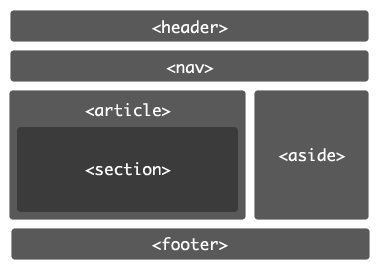
\includegraphics[scale=0.5]{img/html5structure.png}
 \end{center}
\end{frame}

\begin{frame}
 \frametitle{Estructura}
 \begin{center}
    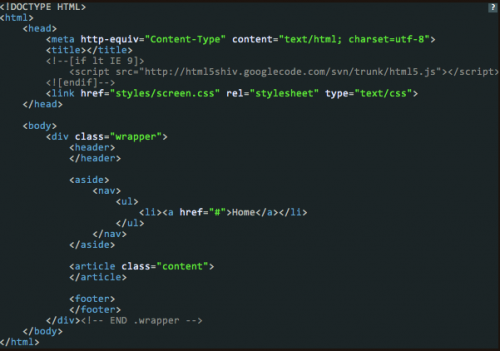
\includegraphics[scale=0.5]{img/html5code.png}
 \end{center}
\end{frame}


\begin{frame}
 \frametitle{Atributos}
 Cada etiqueta tiene atributos específicos, sin embargo, existen un conjunto de atributos comunes a todos los elementos.
 \begin{itemize}
  \item<2-> \alert{id} este atributo debe ser único en el documento y representa el identificador de la etiqueta.
  \item<3-> \alert{class} este atributo permite definir una regla CSS que la etiqueta debe cumplir.
  \item<4-> \alert{style} este atributo permite introducir reglas específico de CSS.
  \item<5-> \alert{title} El título de la etiqueta que se despliega al posar el mouse sobre el elemento.
 \end{itemize}
\end{frame}


\begin{frame}
 \frametitle{Atributos}
 Recuerde \href{http://www.w3schools.com/html/default.asp}{http://www.w3schools.com/html/default.asp} es su amigo.
\end{frame}

\subsection{CSS}

\begin{frame}
 \frametitle{CSS}
 Las Hojas de Estilo en Cascada (Cascading Style Sheets) es el lenguaje de hojas de estilo utilizado para describir el aspecto y el formato de un documento escrito en un lenguaje de marcas, esto incluye varios lenguajes basados en XML como son HTML, XHTML o SVG.
 \newline
 La ventaja es que los estilos se pueden adjuntar en un documento separado o en el mismo documento HTML. En este último caso podrían definirse estilos generales en la cabecera del documento o en cada etiqueta particular mediante el atributo ``style''.
\end{frame}

\begin{frame}
 \frametitle{CSS}
 Una hoja de estilo se compone de una lista de reglas. Cada regla o conjunto de reglas consiste en uno o más selectores y un bloque de declaración (o ``bloque de estilo'') con los estilos a aplicar para los elementos del documento que cumplan con el selector que les precede. 
 Cada bloque de estilos se define entre llaves, y está formado por una o varias declaraciones de estilo con el formato \alert{propiedad: valor;}
\end{frame}


\begin{frame}
 \frametitle{Estructura}
 \begin{center}
    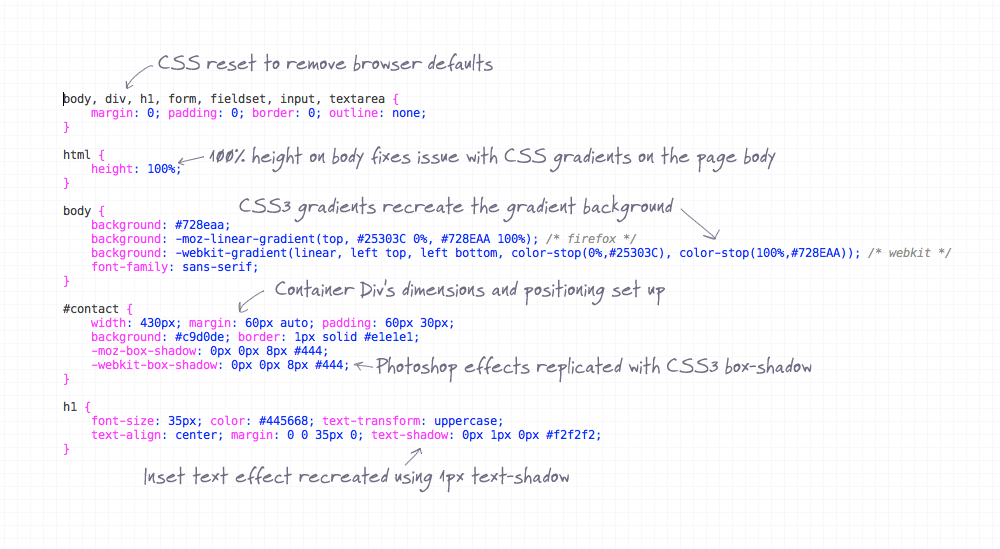
\includegraphics[scale=0.35]{img/css1.png}
 \end{center}
\end{frame}


\section{JavaScript / jQuery}

\section{JavaScript}

\begin{frame}
 \frametitle{JavaScript}
 JavaScript (JS) es un lenguaje de programación interpretado, Orientado a objetos, basado en prototipos, imperativo, débilmente tipado y dinámico.
 \newline
 Se utiliza principalmente en su forma del lado del cliente (client-side), implementado como parte de un navegador web permitiendo mejoras en la interfaz de usuario y páginas web dinámicas.
\end{frame}

\begin{frame}
 \frametitle{JavaScript}
 Al igual que con el código CSS, JavaScript se puede colocar en los sitios web ya sea incrustandolo en el código HTML, con la etiqueta script, o adjuntandolo en un archivo separado.
\end{frame}

\begin{frame}
 \frametitle{Estructura}
 \begin{center}
    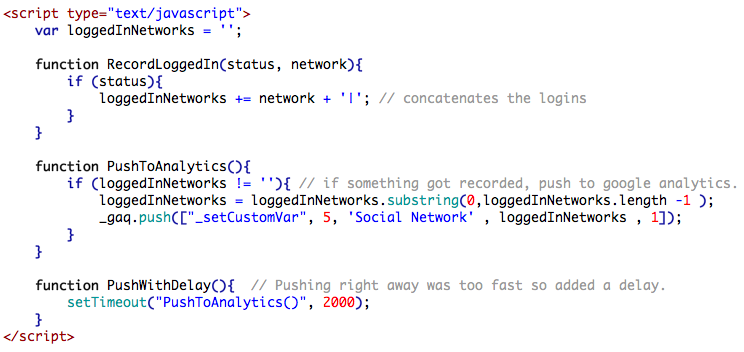
\includegraphics[scale=0.35]{img/js.png}
 \end{center}
\end{frame}


\subsection{jQuery}

\begin{frame}
 \frametitle{jQuery}
 jQuery es una biblioteca de JavaScript, creada inicialmente por John Resig, que permite simplificar la manera de interactuar con los documentos HTML, manipular el árbol DOM, manejar eventos, desarrollar animaciones y agregar interacción con la técnica AJAX a páginas web.
\end{frame}


\begin{frame}
 \frametitle{jQuery}
 Lo que ha hecho de jQuery, tan popular, es la facilidad y belleza que provee para crear funciones y extender las características de JavaScript.
\end{frame}


\section{PHP}

\subsection{PHP}

\begin{frame}
 \frametitle{PHP}
 PHP es un lenguaje de programación de uso general de código del lado del servidor originalmente diseñado para el desarrollo web de contenido dinámico. Fue uno de los primeros lenguajes de programación del lado del servidor que se podían incorporar directamente en el documento HTML en lugar de llamar a un archivo externo que procese los datos. El código es interpretado por un servidor web con un módulo de procesador de PHP que genera la página Web resultante. PHP ha evolucionado por lo que ahora incluye también una interfaz de línea de comandos que puede ser usada en aplicaciones gráficas independientes.
\end{frame}

\begin{frame}
 \frametitle{PHP}
 PHP es un lenguaje interpretado y débilmente tipado. Es muy flexible, puede ser tanto procedural como orientado a objetos. La mayoría de los frameworks usan las características orientadas a objetos.
\end{frame}

\begin{frame}
 \frametitle{Objeto}
 En el paradigma de programación orientada a objetos (POO, o bien OOP en inglés), un objeto es una unidad dentro de un programa que consta de un estado y de un comportamiento, que a su vez constan respectivamente de datos almacenados y de tareas realizables durante el tiempo de ejecución. Un objeto puede ser creado instanciando una clase, como ocurre en la programación orientada a objetos, o mediante escritura directa de código y la replicación otros objetos, como ocurre en la programación basada en prototipos.
\end{frame}

\section{SQL / PostgreSQL}

\subsection{SQL}

\begin{frame}
 \frametitle{SQL}
 El lenguaje de consulta estructurado o SQL (Structured Query Language) es un lenguaje declarativo de acceso a bases de datos relacionales que permite especificar diversos tipos de operaciones en ellas. Una de sus características es el manejo del álgebra y el cálculo relacional que permiten efectuar consultas con el fin de recuperar de forma sencilla información de interés de bases de datos, así como hacer cambios en ellas.
\end{frame}

\subsection{PostgreSQL}

\begin{frame}
 \frametitle{PostgreSQL}
 PostgreSQL es un sistema de gestión de bases de datos, que permiten el almacenamiento, modificación y extracción de la información en una base de datos, además de proporcionar herramientas para añadir, borrar, modificar y analizar los datos. Tiene licencia BSD y es uno de los sistemas más robustos y confiables del mercado.
\end{frame}


\section{Laravel}

\subsection{Laravel}

\begin{frame}
 \frametitle{Laravel}
 Laravel tiene como objetivo ser un framework que permita el uso de una sintaxis elegante y expresiva para crear código de forma sencilla y permitiendo multitud de funcionalidades. Intenta aprovechar lo mejor de otros frameworks (principalmente Symfony) y aprovechar las características de las últimas versiones de PHP.
\end{frame}


\begin{frame}
 \frametitle{Laravel}
 \begin{itemize}
  \item Sistema de ruteo, también RESTful
  \item Blade, Motor de plantillas
  \item Eloquent ORM
  \item Basado en Composer
  \item Soporte para el caché
  \item Soporte para MVC
 \end{itemize}
\end{frame}

\subsection{Instalación del Proyecto}

\begin{frame}
 \frametitle{Instalación}
 Los requisitos de instalación:
 \begin{itemize}
  \item PHP (igual o superior a 5.3.7)
  \item Compilación de PHP con soporte a mcrypt, openssl, y al menos el motor de base de datos a utilizar (en nuestro caso PostgreSQL).
  \item Composer
 \end{itemize}
\end{frame}


\begin{frame}
 \frametitle{Instalación}
 El primer paso es instalar Composer:
 \newline
 {\bf curl -sS https://getcomposer.org/installer \textbar  php}
 \newline
 {\bf sudo mv composer.phar /usr/local/bin/composer}
 \newline
 Con esto deberíamos disponer del comando composer dentro de nuestro path
\end{frame}


\begin{frame}
 \frametitle{Instalación}
 En un terminal, ubicarse en una carpeta adecuada y ejecutar:
 \newline
 {\bf composer create-project laravel/laravel proyecto-laravel --prefer-dist}
 \newline
 Con dicho comando deberíamos crear un proyecto, de nombre ``proyecto-laravel''.
\end{frame}


\begin{frame}
 \frametitle{Estructura del proyecto}
 \begin{itemize}
  \item<2-> \alert{/app} Contiene los controladores, modelos, vistas y configuraciones de la aplicación. En esta carpeta escribiremos la mayoría del código para que nuestra aplicación funcione.
  \item<3-> \alert{/public} Es la única carpeta a la que los usuarios de la aplicación pueden acceder. Todo las peticiones y solicitudes a la aplicación pasan por esta carpeta, ya que en ella se encuentra el index.php, este archivo es el que inicia todo el proceso de ejecución del framework. En este directorio también se alojan los archivos CSS, Javascript, imágenes y otros archivos que se quieran hacer públicos.
  \item<4-> \alert{/vendor} En esta carpeta se alojan todas las librerías que conforman el framework y sus dependencias.
 \end{itemize}
\end{frame}


\begin{frame}
 \frametitle{Estructura del proyecto}
 \begin{itemize}
  \item<2-> \alert{/lang} En esta carpeta se guardan archivos PHP que contienen Arrays con los textos de diferentes lenguajes, en caso que se desee que la aplicación se pueda traducir.
  \item<3-> \alert{/app/config} Aquí se pueden se pueden encontrar todos los archivos de configuración de la aplicación. Base datos, cache, correos, sesiones o cualquier otra configuración general de la aplicación.
  \item<4-> \alert{/app/controller} Contiene todos los archivos con las clases de los controladores que sirven para interactuar con los modelos, las vistas y manejar la lógica de la aplicación.
 \end{itemize}
\end{frame}


\begin{frame}
 \frametitle{Estructura del proyecto}
 \begin{itemize}
  \item<2-> \alert{/app/model} Los modelos son clases que representan la información (datos) de la aplicación y las reglas para manipularlos. En la mayoría de los casos cada tabla de la base datos esta representada con un modelo. La lógica de negocio de la aplicación esta contendía en los modelos.
  \item<3-> \alert{/app/views} Este directorio contiene las plantillas de HTML que usan los controladores para mostrar la información. Hay que tener en cuenta que en esta carpeta no van los Javascript, CSS o imágenes, ese tipo de archivos van alojados en la carpeta /public.
 \end{itemize}
\end{frame}


\begin{frame}
 \frametitle{Configuración de la Base de datos}
 Dentro de la carpeta de instalación se debe configurar el archivo /app/config/database.php
 \begin{center}
    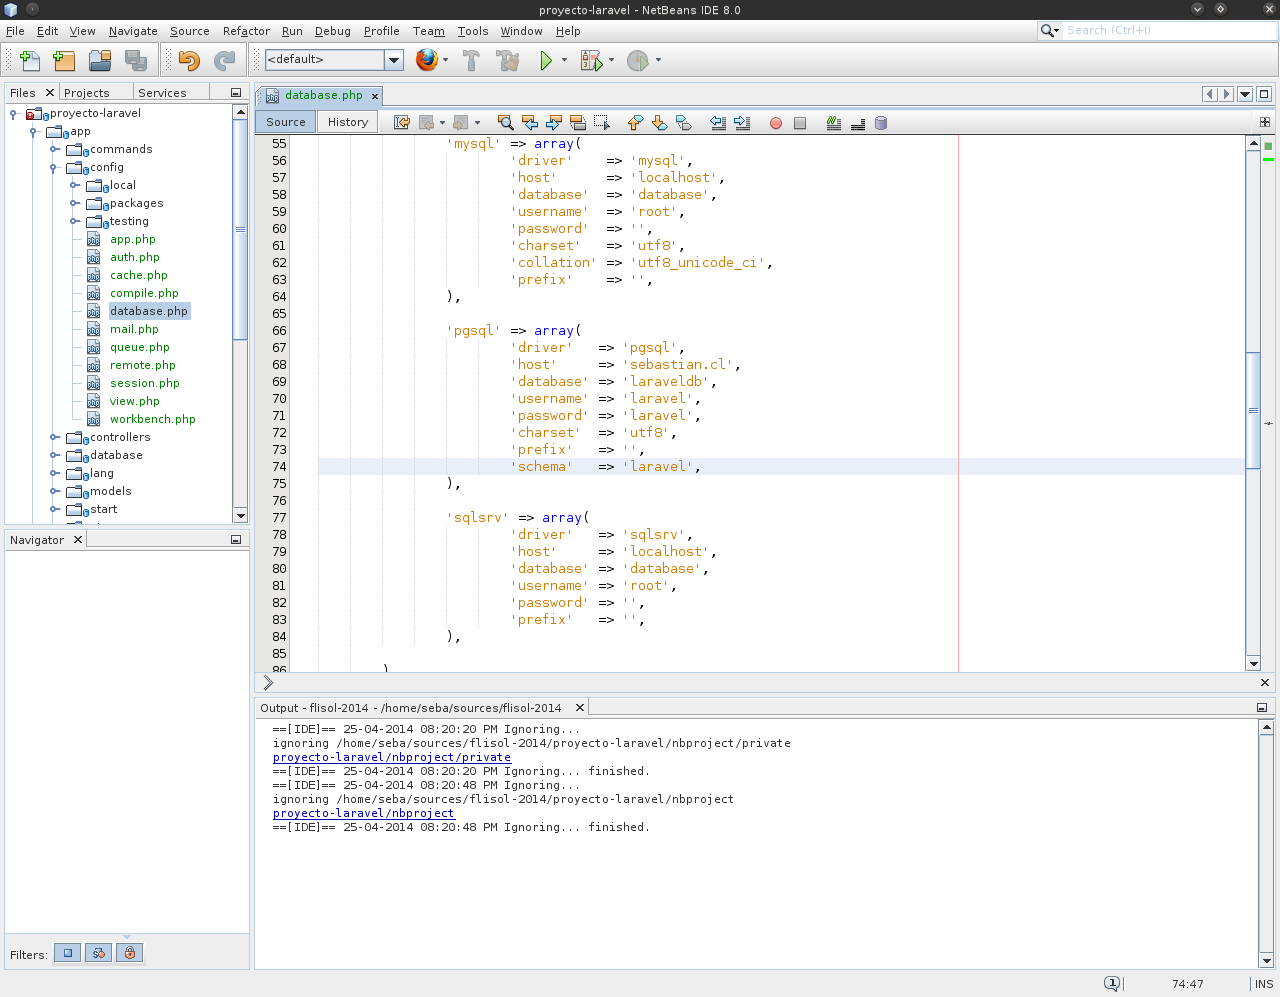
\includegraphics[scale=0.35]{img/databasephp.png}
 \end{center}
\end{frame}

\begin{frame}
 \frametitle{Configuración}
 También hay que configurar:
 \begin{itemize}
  \item /app/config/app.php
  \item /app/config/mail.php
  \item /app/config/session.php
 \end{itemize}
\end{frame}

\subsection{Modelando el Proyecto}

\begin{frame}
 \frametitle{Modelo}
 Existe básicamente dos opciones para crear el modelo del proyecto:
 \begin{itemize}
  \item Usar ``migraciones'' (crear clases que se transformarán en tablas).
  \item Modelar desde la Base de datos. (Crear las tablas primero, y en base a estas desarrollar el modelo).
 \end{itemize}
 En mi opinión, es mejor desarrollar un buen modelo de base de datos, y crear el modelo a partir del modelo.
\end{frame}


\begin{frame}
 \frametitle{Modelo}
 Para este taller crearemos un pequeño modelo con 3 tablas.
 \begin{center}
    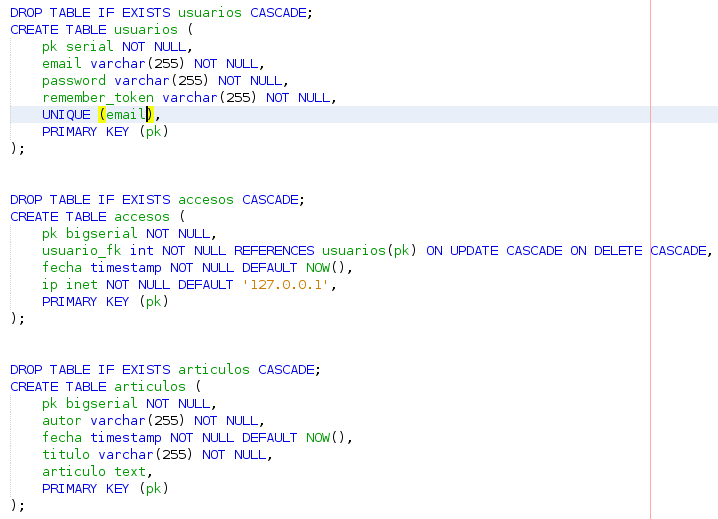
\includegraphics[scale=0.45]{img/modelo.png}
 \end{center}
\end{frame}

\begin{frame}
 \frametitle{Modelo}
 El siguiente paso, es llevar este modelo de base de datos, a un modelo de objetos PHP que podamos usar con laravel.
 \begin{center}
    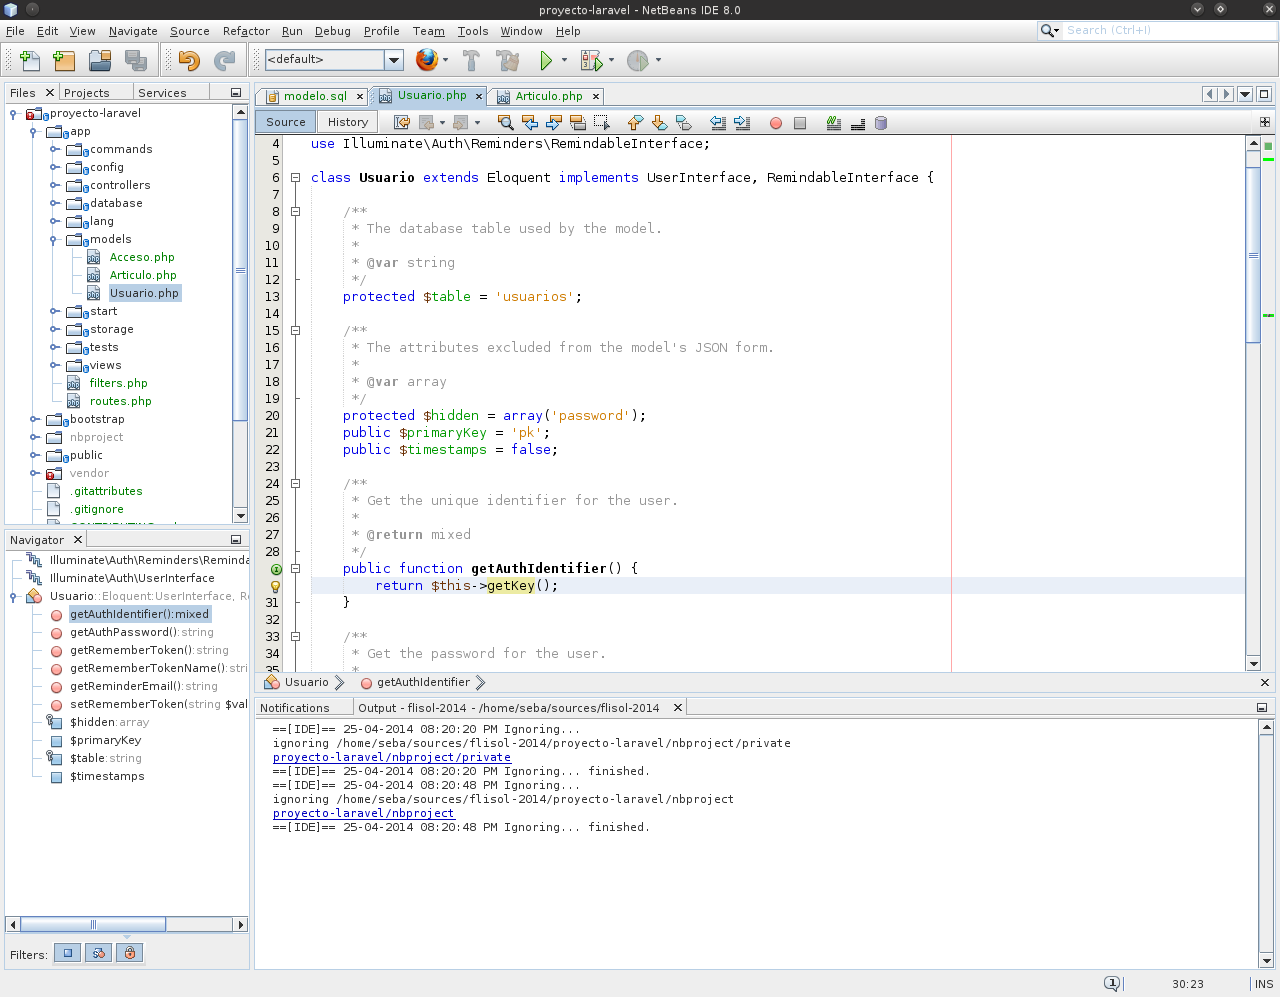
\includegraphics[scale=0.3]{img/modelo_poo.png}
 \end{center}
\end{frame}

\begin{frame}
 \frametitle{Modelo}
 Después de crear el modelo, se debe ejecutar:
 \newline
 {\bf composer dump-auto}
 \newline
 Esto es importante, ya que de no ejecutar este comando, el framework no autocargará las clases nuevas.
\end{frame}



\begin{frame}
 \frametitle{Plantillas}
 Es importante disponer de un diseño web bonito, atractivo y acabado, cuál proyecto interesante debe ser visualmente atractivo.
 Un buen lugar para comenzar es utilizar un template basado en:
 \newline
 http://html5boilerplate.com/
\end{frame}


\begin{frame}
 \frametitle{Plantillas}
 Crearemos una carpeta ``layouts'', dentro de /app/views, que será la base de donde almacenaremos nuestras plantillas.
 \newline
 En nuestro ejemplo crearemos un archivo main.blade.php dentro de la carpeta layouts basado en el index.html generado por html5boilerplate. También colocaremos los css, js y archivos auxiliares dentro de /public
 \newline
 En la carpeta /app/views generaremos los archivos necesarios, para que nuestros propósitos
\end{frame}

\begin{frame}
 \frametitle{Creación de Controlador}
 Podemos crear controladores automáticamente usando el siguiente comando en la carpeta base del proyecto:
 \newline
 {\bf php artisan controller:make ArticuloController}
\end{frame}



\subsection{Rutas}

\begin{frame}
 \frametitle{Rutas}
 \begin{center}
    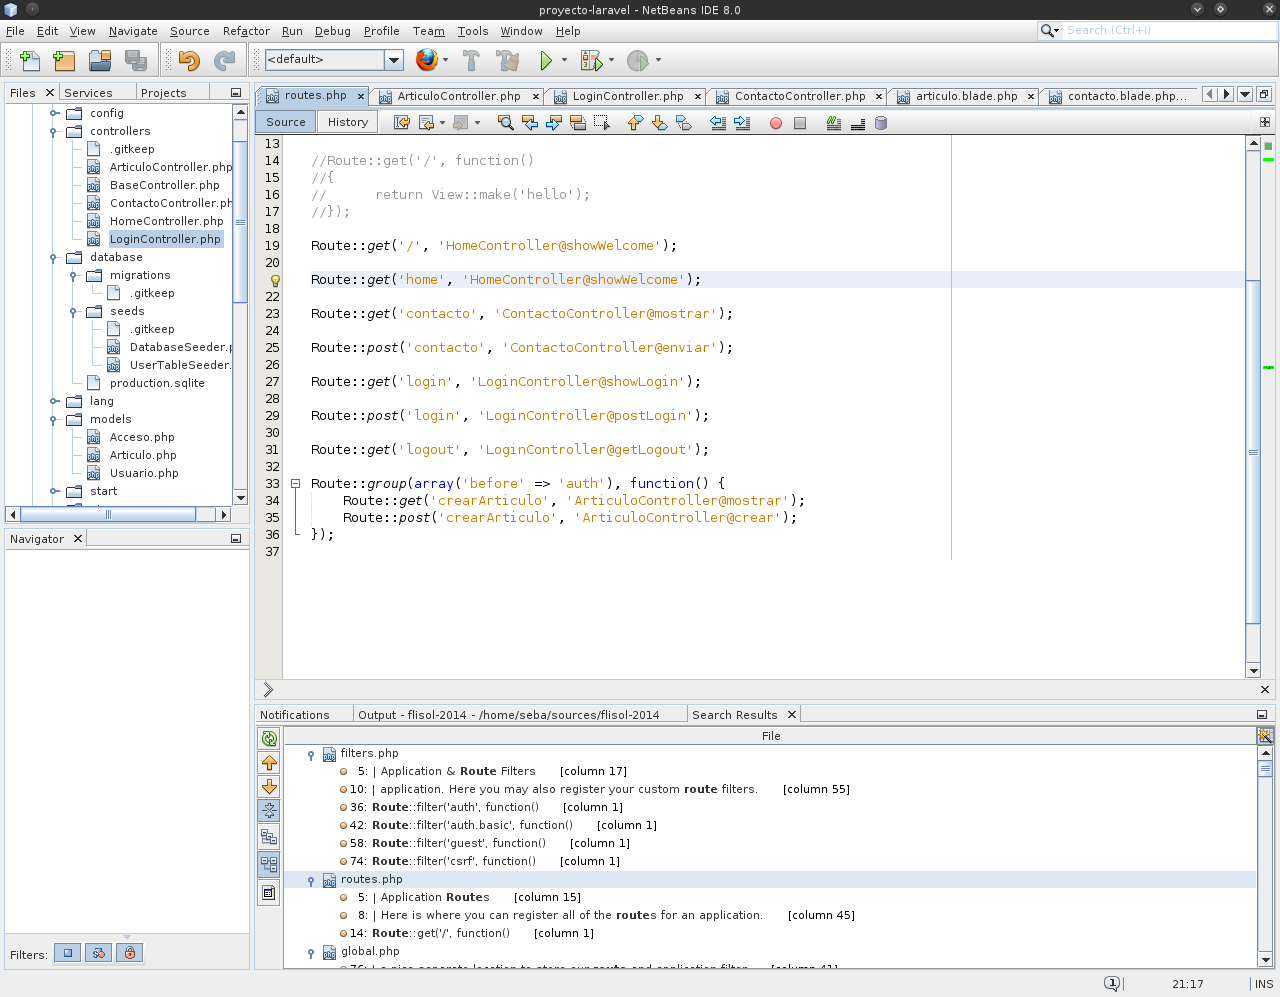
\includegraphics[scale=0.3]{img/rutas.png}
 \end{center}
\end{frame}



\section{TODO}

\begin{frame}
 \frametitle{TODO}
 Mejorar el diseño Gráfico, agregar un sistemas de comentarios, aumentar la funcionalidad.
\end{frame}


\frame{
  \vspace{2cm}
  {\huge ¿ Preguntas ?}

  \vspace{3cm}
  \begin{flushright}
    Sebastián Salazar Molina

    \structure{\footnotesize{@sebastian\_sm}}
  \end{flushright}
}

\end{document}
